%%%%%%%%%%%%%%%%%%%%%%%%%%%%%%%%%%%%%%%%%%%%%%%%%%%%%%%%%%%%%%%%%%
%%%%%%%% ICML 2015 EXAMPLE LATEX SUBMISSION FILE %%%%%%%%%%%%%%%%%
%%%%%%%%%%%%%%%%%%%%%%%%%%%%%%%%%%%%%%%%%%%%%%%%%%%%%%%%%%%%%%%%%%

% Use the following line _only_ if you're still using LaTeX 2.09.
%\documentstyle[icml2015,epsf,natbib]{article}
% If you rely on Latex2e packages, like most moden people use this:
\documentclass{article}
\usepackage{pdflscape}
\usepackage{tabularx}
\usepackage{lipsum}
\usepackage{amsmath,array}
\usepackage{kantlipsum}
\usepackage{float}
% use Times
\usepackage{times}
% For figures
\usepackage{graphicx} % more modern
%\usepackage{epsfig} % less modern
\usepackage{subfigure} 

% For citations
\usepackage{natbib}

% For algorithms
\usepackage{algorithm}
\usepackage{algorithmic}

% As of 2011, we use the hyperref package to produce hyperlinks in the
% resulting PDF.  If this breaks your system, please commend out the
% following usepackage line and replace \usepackage{icml2015} with
% \usepackage[nohyperref]{icml2015} above.
\usepackage{hyperref}

% Packages hyperref and algorithmic misbehave sometimes.  We can fix
% this with the following command.
\newcommand{\theHalgorithm}{\arabic{algorithm}}

% Employ the following version of the ``usepackage'' statement for
% submitting the draft version of the paper for review.  This will set
% the note in the first column to ``Under review.  Do not distribute.''
%\usepackage[accepted]{icml2015} 

% Employ this version of the ``usepackage'' statement after the paper has
% been accepted, when creating the final version.  This will set the
% note in the first column to ``Proceedings of the...''
\usepackage[accepted]{icml2015}


% The \icmltitle you define below is probably too long as a header.
% Therefore, a short form for the running title is supplied here:
\icmltitlerunning{Sentimental analysis for yelp dataset}

\begin{document} 





\twocolumn[
\icmltitle{Sentimental analysis for yelp dataset}


% It is OKAY to include author information, even for blind
% submissions: the style file will automatically remove it for you
% unless you've provided the [accepted] option to the icml2015
% package.
\icmlauthor{Bhaskar Jupudi}{njupudi@ucsc.edu}
\icmlauthor{Trivikram Bollempalli}{tbollemp@ucsc.edu}
\icmlauthor{Chandrahas}{cjagadis@ucsc.edu}
\icmlauthor{Karthikeyan}{karthik@ucsc.edu}
\icmlauthor{GitHub Link}{https://github.com/jupudibhaskar967/CMPS-242-Project.git}

% You may provide any keywords that you 
% find helpful for describing your paper; these are used to populate 
% the "keywords" metadata in the PDF but will not be shown in the document
\icmlkeywords{boring formatting information, machine learning, ICML}
\vskip 0.3in
]




\begin{abstract} 
In this project, we aim to perform sentiment analysis i.e., classifying whether the review is postive or negative using the yelp dataset based on reviews and ratings. The classification problem can be solved by a set of algorithms. Every algorithm has its own advantages and disadvantages in terms of accuracy and model complexity. 

For example, Naive Bayes classifier is faster to compute than Logistic Regression classifier for huge datasets. But the disadvantage with the former is that it assumes that features are independent where as the latter has no such assumptions which can lead to better precdiction. Our work mainly concentrates on implementing these two classifiers and techniques to make them perform much better. We have adopted multi-processing for feature extraction to make it way faster and also implemented two different approaches of Logistic regression for both binary and multi-class classfication. We have also implemented Naive Bayes classifier. Finally, we contrast these two algorithms based on time taken for execution and performance metrics like accuracy, precision and recall. 
\end{abstract} 

\section{Problem statement}


\section{Feature Extraction}

We have extracted the features for respective algorithms using our own constraints and formulations instead of using count vectorizer. The reason we designed this because countvectorizer method is raising a run-time exception for a large dataset (\textgreater300k reviews).

\subsection{Binary classification}
For logistic regression, we need to form a data vector from a bag of words which contains the word count. To compute this, first we extracted 4/5 th of our total dataset (which is our training data) and extracted the words and their respective counts into a dictionary. Out of all these words, we have used three constraints to restrict the number of bag of words. One, if a word occurs for 'x' times in a positive review then we considered that word into bag of words only if the same word occurs for less than 4/10 th times in the negative review and vice-versa. Second, total word count for a specific word should be more than 14. Third, we check if length of the word is more than 2 characters thereby restricting the number of features to 8895. The exact numbers we have used is just an arbitrary choice and can vary to adjust the accuracy. The intuition behind this is, a word which have equal count over both postive and negative reviews and if a word occurs over all the reviews for very less frequent times (\textless10 or so which might be a typing mistake) will be having a very less impact over the decision rule and single character words may not effect the meaning of the review when considered as a whole.

After obtaining bag of words, we formed data vector 'x', using multi-processing (as it is both compute and memory intensive operation) to make it more faster as each review can be formed into a count vector indepedently. For this we have used multiprocessing.Pool library in python. We used pool.map\_async() method to make all the individual vectors into a single data vector. 

For Naive Bayes algorithm, we directly used all the words in the initial dictionary without using any constraints as there is no requirement for us to form the data vector as we did in logistic regression and the computation is way faster because of the assumption that features are independent of each other. 


\subsection{Multiclass classification}

For logistic regression, we did not use the same constriants as we did earlier because there are multiple classes instead of 2. Alternatively, we have selected most frequent 10k words from the dictionary after extracting the reviews. Later, we have formed the data vector 'x' in the same way as above using multi-processing.   

We did the same thing for Naive Bayes algorithm, as we did in the binary classification.

\section{Model Formulation}
From Feature Engineering, we get input data and its labels. we will use this to train our logistic regression algorithm. We have implemented both logistic regression for two classes and also multi-class logistic regression.
\subsection{Binary Logistic Regression}
\begin{equation}
P(C_{1}|X) = \vspace{10mm}   \frac{p(X|C_{1}).p(C_{1})}{p(X|C_{1}).p(C_{1}) + p(X|C_{2}).p(C_{2})}
\end{equation}

The probability for the first class is given by 
\begin{equation}
P(C_{1}|X) = y(x)  = \sigma(W\textsuperscript{T}X + b) 
\end{equation}
The likelihood is given as 
\begin{equation}
P(t|W) = \prod\limits_{n=1}^N (y_{n})^{t_{n}}(1-y_{n})^{1- t_{n}}
\end{equation}

The cost function is 
\begin{equation}
E(w) = -ln \hspace{1mm} p(t|W) = -\sum\limits_{n=1}^N t_{n}\hspace{1mm}ln(y_{n}) + (1-t_{n})ln(1-y_{n})
\end{equation}

Gradient is calculated as follows
\begin{equation}
\nabla E(w) = \sum\limits_{n=1}^N (y_{n} - t_{n}) \phi_{n}
\end{equation}



\subsection{Multiclass Logistic regression}
The probability of a class in logistic regression with multiple classes is given by:
p (Ck |x) = yk (φ) = exp (ak ) P j exp (aj) where ak = ln p (x|Ck ) + ln p (Ck )
We estimated the parameters using Maximum Log Likelihood estimation. For N data points, the likelihood function is : 
= Y N n=1 Y K k=1 y tnk nk
Taking log on both sides and negation of it, we get the below negative log likelihood function:
X N n=1 X K k=1 tnk ln ynk
E(w) is our cost function which we want to minimize to estimate W parameters. The gradient for the cost function is given by:
∇E (w1, . . . , wK ) = X N n=1 (ynj − tnj) φn
We use this gradient in minimizing the cost function.

\subsection{Optimization techniques}
We used fmin\_l\_bfgs\_b and stochastic gradient descent to minimize the cost function and obtain W. fmin\_l\_bfgs\_b is from scipy.optimize module in python. It uses the gradient that we calculated above in minimizing the cost function.

We also implemented Stochastic Gradient Descent(SGD). SGD is similar to gradient descent algorithm. In gradient descent, we find gradient for the entire training dataset and then update W using W = W - alpha*gradient(w,x,y). Here alpha is the learning rate, W is the weight vector, x,y are training data. At each step, gradient descent update W, hoping that it minimizes the cost function. This is true as long as we choose proper alpha and gradient descent converges close to global minimum since the cost function is convex. In SGD, w is updated by finding gradient over each sample. We can also find gradient over a batch of training data which is a compromise between the two extremes. Finding gradient over a batch increases performance compared to single example because python can use the underlying vectorization libraries. We have implemented SGD in this way where you can specify batch size.

\section{Evaluations}

We performed all our experiments on a server that has 24 physical cores (with hyperthreading 2) and 128GB of DRAM. We are testing our binary and multinomial logistic regression algorithms on yelp dataset. We are using three metrics viz., Accuracy, Precision, Recall to evaluate these algorithms. These three metrics are calculated as follows.


Accuracy = (number of correctly classified test cases) / (total number of test cases) 


Precision = (true positives) / (true positives + false positives)


Recall =  (true positives) / (true positives + false negatives)


We also compare the performance of our logistic regression algorithm with naive bayes approach, which we implemented from scratch and discuss tradeoffs. We compare the performance of logistic regression when fmin\_l\_bfgs\_b and Stochastic Gradient Descent are used as optimizers.

\section{Results}


\subsection{Effect of parallelism}
We implemented multi-processing to compute the feature vector in order to make it faster as it is a compute intensive operation. The following table is drawn to illustrate the time taken for extracting the features from data of size 100k and 50k reviews. With parallelism, we are able to achieve it in approximately 1/10 th of the total time without parallelism.


\begin{table}[H]
\caption{Execution time for extraction of features in Logistic regression classifier.}
\label{sample-table}
\begin{center}
\begin{small}
\begin{sc}
\begin{tabular}{lllll}
\hline
Parallelism & Size & Features & Time \\
\hline
No  & 100k & 9049 & 65m36.271s \\
No  & 50k & 5323 & 18m32.441s \\
Yes  & 100k & 9049 & 7m8.291s \\
Yes  & 50k & 5323 & 2m36.947s \\
\hline
\end{tabular}
\end{sc}
\end{small}
\end{center}
\end{table}


As explained earlier, we have designed our feature extraction algorithm because the built-in function countvectorizer() is throwing a run-time exception for a huge dataset which is beyond 300k reviews.


\begin{table}[H]
\caption{Parallelism vs countvectorizer()}
\label{sample-table}
\begin{center}
\begin{small}
\begin{sc}
\begin{tabular}{lllll}
\hline
Method & Features & Time \\
\hline
Parallel  & 17083 & 42m27.394s \\
countvectorizer  & 10k & Run-Time error \\
\hline
\end{tabular}
\end{sc}
\end{small}
\end{center}
\end{table}



\subsection{Comparision of LR and NB}
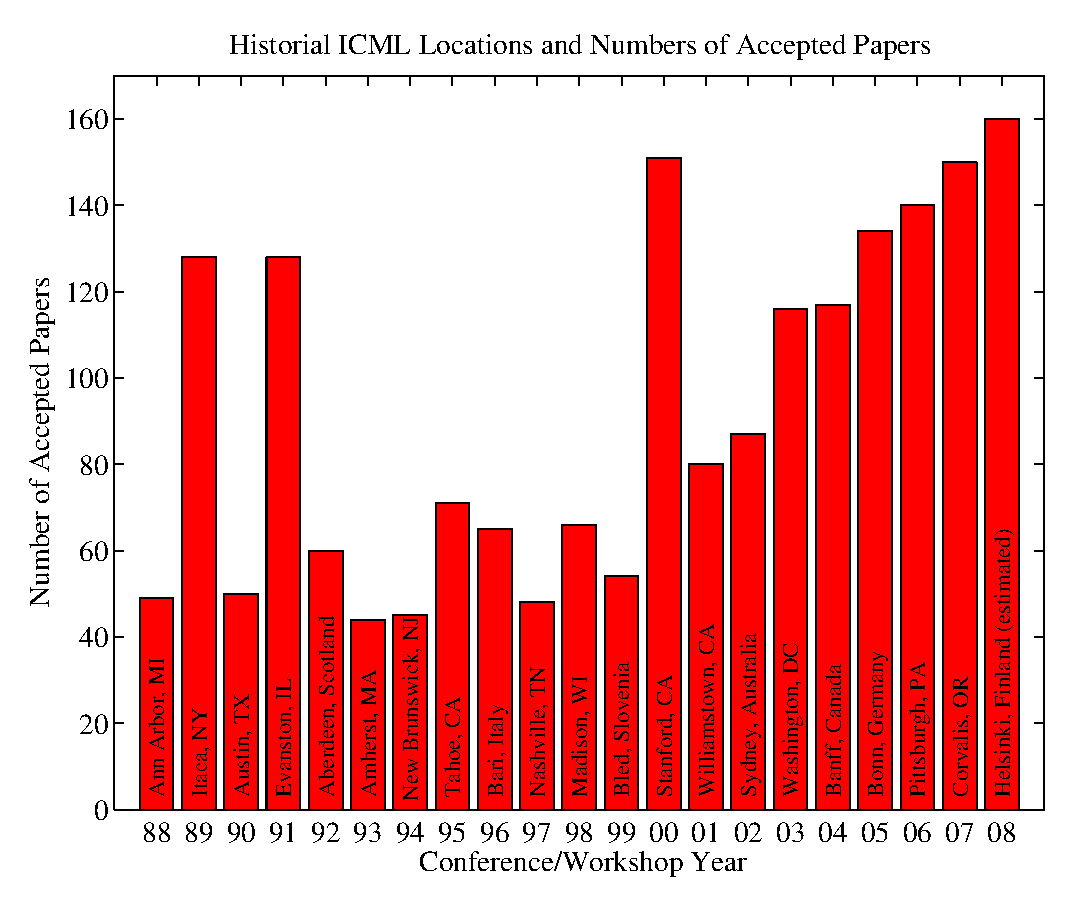
\includegraphics[width=0.5\textwidth]{icml_numpapers}



\section{Conclusion}
% In the unusual situation where you want a paper to appear in the
% references without citing it in the main text, use \nocite
\nocite{langley00}

\bibliography{example_paper}
\bibliographystyle{icml2015}

\end{document} 


% This document was modified from the file originally made available by
% Pat Langley and Andrea Danyluk for ICML-2K. This version was
% created by Lise Getoor and Tobias Scheffer, it was slightly modified  
% from the 2010 version by Thorsten Joachims & Johannes Fuernkranz, 
% slightly modified from the 2009 version by Kiri Wagstaff and 
% Sam Roweis's 2008 version, which is slightly modified from 
% Prasad Tadepalli's 2007 version which is a lightly 
% changed version of the previous year's version by Andrew Moore, 
% which was in turn edited from those of Kristian Kersting and 
% Codrina Lauth. Alex Smola contributed to the algorithmic style files.  
\grid
